%\documentclass{svjour3}                     % onecolumn (standard format)
%\documentclass[smallcondensed]{svjour3}     % onecolumn (ditto)
\documentclass[smallextended]{svjour3}       % onecolumn (second format)
%\documentclass[twocolumn]{svjour3}          % twocolumn
%
\smartqed  % flush right qed marks, e.g. at end of proof
%
\usepackage{graphicx}
%
% \usepackage{mathptmx}      % use Times fonts if available on your TeX system
%
% insert here the call for the packages your document requires
%\usepackage{latexsym}
% etc.
%
% please place your own definitions here and don't use \def but
% \newcommand{}{}
%
% Insert the name of "your journal" with
 \journalname{Computing}
%

%%% User-requested packages placed after this line %%%%%%%%%%%%%%%%%%%%%%%%%%%%
\usepackage{amsfonts,amssymb,amsmath}
\usepackage{booktabs,dcolumn}
\usepackage[T1]{fontenc}
\usepackage{mathtools}
\usepackage{enumerate,graphicx}
\usepackage{subfig}
\usepackage{multirow}
\usepackage{listings}
\usepackage{xcolor}
\usepackage[numbers,sort&compress]{natbib} 

% \usepackage[center]{subfigure}
\numberwithin{equation}{section}
\usepackage{braket}                             %Provides \Set for typing sets
\usepackage{float} 
\usepackage{subfig}

%%% User's macros placed after this line %%%%%%%%%%%%%%%%%%%%%%%%%%%%%%%%%%%%%%
%\IfFileExists{dsfont.sty}%
%\usepackage{dsfont}
\newcommand{\R}{\mathbb{R}}
\newcommand{\N}{\mathbb{N}}
\renewcommand{\phi}{\varphi}
\renewcommand{\epsilon}{\varepsilon}
\newcommand{\deal}{\texttt{deal.II}}
\newcommand{\dope}{\texttt{DOpElib}}
\newcommand{\re}{\operatorname{Re}}



%\newcommand{\todo}[1]{\textbf{\textsc{\textcolor{black}{TODO: #1}}}}
\newcommand{\todo}[1]{\textbf{\textsc{\textcolor{blue}{TODO: #1}}}}
\newcommand{\todocg}[1]{\textbf{\textsc{\textcolor{red}{TODO: #1\textasciitilde cg}}}}
\newcommand{\todoww}[1]{\textbf{\textsc{\textcolor{green}{TODO: #1\textasciitilde ww}}}}
%\newcommand{\mymarginpar}[1]{\marginpar{\textcolor{red}{\scriptsize{#1}}}}
\newcommand{\mymarginpar}[1]{\marginpar{\textcolor{red}{\normalsize{#1}}}}
%

\begin{document}


\title{DOpElib: Differential Equations and Optimization Environment; A Goal Oriented Software Library for Solving PDEs and Optimization Problems with PDEs}


\titlerunning{DOpElib}        % if too long for running head

\author{C. Goll \and T. Wick \and W. Wollner}

%\authorrunning{Short form of author list} % if too long for running head

\institute{Christian Goll \at
              Institute of Applied Mathematics, University of Heidelberg
              \\Im Neuenheimer Feld 293/294, 69120 Heidelberg, Germany\\
              %Tel.: +49 622-154-6154\\
              \email{cgoll@iwr.uni-heidelberg.de}           %  \\
           \and
Thomas Wick \at
              The Institute for Computational Engineering and Sciences,\\
The University of Texas at Austin,\\
Austin, Texas 78712, USA \\
              %Tel.: +1 512-672-7763\\
              \email{twick@ices.utexas.edu}   
 \and
Winnifried Wollner \at
              Universit\"at Hamburg\\
              Department of Mathematics\\
              Bundesstr. 55, 20146 Hamburg, Germany\\
              \email{winnifried.wollner@math.uni-hamburg.de}   
}

\date{Received: date / Accepted: date}
% The correct dates will be entered by the editor

%%%%%%%%%%%%%%%%%%%%%%%%%%%%%%%%%%%%%%%%%%%

\maketitle

%%%%%%%%%%%%%%%%%%%%%%%%%%%%%%%%%%%%%%%%%%%
\begin{abstract}
In this article, we describe the  
\textit{Differential Equations and Optimization Environment} (\dope{}).
\dope{} is a software library that provides a unified interface 
to high level algorithms such as time-stepping methods, nonlinear solvers and 
optimization routines. This structure ensures 
that, first of all, the user is only required to write those sections of code 
that are specific to 
the considered problem. Second, the exchange of parts of the used routines is possible 
with only a few lines of code to change instead of large reimplementations.
The article illustrates the design principles and various features
of \dope{} and provides some 
numerical results as demonstration for the versatility of the software.
\end{abstract}
%%%%%%%%%%%%%%%%%%%%%%%%%%%%%%%%%%%%%%%%%%%
\section{Introduction}
\label{introduction}
Today, there exists a broad variety of software libraries
that provide numerical tools for solving partial differential
equations (PDEs). Prominent examples are 
\deal{} \citep{dealnew}, dune \citep{dune}, 
FEniCS \citep{fenics}
or commercial solvers as for instance ANSYS (with its Fluent package),
COMSOL, or simufact forming.
Finally, a lot of work is (still) done in Matlab.
In fact, these libraries provide very useful tools 
for a huge variety of applications. 

In many cases, the user is confronted with 
certain bottlenecks when using such software. 
On the one hand, in open-source projects for academic research, 
standard high-level routines 
which are necessary to solve even simplest PDEs,
such as linear and nonlinear solvers or time-stepping schemes must 
be implemented by the users themselves. However, such routines are, at large,
problem-independent and could be provided as standard tools. 
As our guiding design principle, we note that in many 
numerical studies, the main task is the computation of some  
target functional, e.g., error norms,
point values, or certain mean-values such as drag or lift coefficients.
As a second motivating principle, 
there is nowadays an increasing interest in solving
optimization problems in which the state equation is governed 
by a PDE. Such optimization problems comprise optimal control,
parameter estimation, inverse problems or optimal experimental design. 
To do this in complex applications requires tremendous work already
on the PDE itself before considering optimization of the processes modeled 
by the PDE. Thus it is advantageous to have an environment that allows to 
focus on the development of an appropriate code for the PDE at first but 
asserts due to the required interface, that the code written for the PDE
is then reusable for the application of state-of-the-art optimization 
routines.

On the other hand, commercial finite element (FE) toolkits provide these 
previously mentioned routines but limits user-interaction
with the source code to an extend that typically conflicts
with the consideration of problems deviating from the intended 
user-base for the commercial product. 
This is quite unsatisfactory because in the development of 
novel numerical algorithms  or in the solution of more complex 
applications the researcher needs to be enabled 
to change certain parameters or pieces of source code. 

This article will provide information on who the {\em Differential 
Equations and Optimization Environment} \dope{}  \cite{dope} 
solves these problems by providing a well structured interface for high-level 
routines integrated
with tools to solve PDEs. At the present stage we provide an interface to 
the finite element library \deal{} and a collection of algorithms to solve
both pure PDE problems as well as optimization problems 
constrained by a PDE. 
This provides an extension to the 
very few tools available doing so; 
successful in-house code examples are Gascoigne \cite{gascoigne}
and RoDoBo \cite{rodobo}. 
Like \dope{}, both have been initiated as well in 
the Numerical Analysis Group in Heidelberg.

The main feature of \dope is to give a unified interface to high level 
algorithms such as 
time-stepping methods, nonlinear solvers and optimization routines. 
\dope{} is designed in such a way that the user only needs to write those parts
of the code that are problem dependent while all invariant 
parts of the algorithms
are reusable without any need for further coding.
In particular, the user is enabled to switch between various different 
algorithms without the need to rewrite the problem dependent code, 
though obviously he or she will
have to replace the algorithm object with an other one. 
This replacement can be done by replacing the appropriate object at only
one point in the code.

While \deal{} --which at present is the only FE-toolkit to which we provide an 
interface-- leaves the implementation of all high-level algorithms to the user, 
\dope{} is user-focused by delivering
prefabricated tools which requires adjustments by the user only for parts
connected to his specific problem. The possible solution of 
optimization problems with PDE constraints is an innovative feature in \dope{}.

To give a brief overview, at the present stage of the development 
the following key features are supported by the library
\begin{itemize}
\item Solvers for nonlinear stationary and nonstationary PDEs in 1d, 2d, and 3d.
\item Various, easily exchangeable, 
  time-stepping schemes (based on finite differences), 
  such as forward Euler, backward Euler,
  Crank-Nicolson, shifted Crank-Nicolson, and Fractional-Step-$\Theta$ scheme.
\item Use of all finite elements of from \deal{} including hp-support.
\item Several examples showing the solution of PDEs including
   Poisson, Navier-Stokes, Plasticity and fluid-structure interaction problems. 
\item Line search and trust region Newton algorithms for the 
   solution of optimization problems with PDE constraints by elimination of 
   the state variable.
\item Interface to SNOPT for the solution of optimization problems with PDEs and
  additional other control and state constraints.
\item Several examples showing how to solve various kinds of optimization 
  problems involving stationary and nonstationary PDE constraints.
\item Goal-oriented mesh adaptation with the Dual Weighted Residual method and
  standard residual based error estimators.
\item Different spatial triangulations for control and state variables without
  the need to reimplement the user dependent code when switching from one common 
  triangulation to different ones.
\end{itemize}

The article is organized as follows. In the main Section
\ref{detailed_description}, a detailed description of 
the main features is given. First, we first explain the solution 
of stationary PDEs, in Section~\ref{subsubsec:stationary problems}, nonstationary PDEs, in Section~\ref{sec:timedep}, and optimization problems, in 
Section~\ref{sec:opt}. 
In all three cases we first described how the interface is designed, and why 
it is designed as such. Then the implementation required by the user is 
demonstrated at an example.
Finally, additional features are discussed in Section~\ref{sec:additional}. 
In the final Section
\ref{applications}, we give three different numerical 
examples which illustrate the versatile features of \dope{}. 



%%%%%%%%%%%%%%%%%%%%%%%%%%%%%%%%%%%%%%%%%%%
\section{Detailed Description of the Main Features}
\label{detailed_description}
This library is designed to allow easy implementation for the numerical solution 
of problems involving PDEs.
By providing interfaces to existing FE-toolkits, at present \deal{}, 
we remove all tedious routine implementation needed in 
\deal{} by introducing appropriate classes that take care of all the 
problem independent implementation while leaving only the problem specific 
parts to the user. To show how this is designed, we will, in the sequel, 
describe the reasoning, first, for a simple stationary PDE, in 
Section~\ref{subsubsec:stationary problems}, and then show
how this idea extends to non stationary problems, in 
Section~\ref{sec:timedep}, as well as to optimization
problems with PDE constraints in, Section~\ref{sec:opt}. 

\subsection{Solving Stationary PDEs}
\label{subsubsec:stationary problems}
For the start, we consider a prototypical problem given by the solution of 
a stationary PDE, which we assume to be given in weak form.
In abstract notation it reads; find some $u$ in an appropriate set
such that
\begin{align}\label{eq:prototype_weak}
a(u)(\phi) = (f,\phi) \quad \forall \phi \in V,
\end{align}
with some suitable space $V$ for the test functions and a 
right hand side function $f$.
To illustrate this further, we take the stationary 
incompressible Navier-Stokes equations in a domain $\Omega \subset \R^d$, 
i.e., $u = (v,p)$ and $\phi = (\phi_u,\phi_p)$ then
\begin{align}\label{eq:ns}
a(u)(\phi) = \nu(\nabla v, \nabla\phi_u) + (v \nabla v,\phi_u) + (p, \nabla \cdot \phi_u) + (\nabla \cdot v ,\phi_p)
\end{align}
for all $\phi \in V = H^1_0(\Omega;\R^d) \times L^2_0(\Omega)$.
Here $(\cdot,\cdot)$ denotes the $L^2$-inner-product.
The solution will be searched for in $V + (u_d,0)$ where $u_d$ is some 
continuation of the given Dirichlet boundary data.
In a typical calculation, we do not only want to calculate $u$ but more likely we are 
interested in one (or several) functionals depending on the solution, i.e., some numbers $J(u)$.

In order to solve this problem, i.e., calculate a sequence of values $J(u_h)$ approximating $J(u)$,
we need to discretize 
the equation. In \dope, we are using finite elements, as they are 
provided by \deal{}, to do this. This means we need to pick a 
subdivision $\mathcal T_h$, for instance into quadrilaterals,
of the domain $\Omega$ and a finite element. In the concrete case, we could, 
for instance, take the inf-sup stable  $\mathcal Q_2/\mathcal Q_1$ 
Taylor-Hood element.
As it is clear, that the initialization of the unknowns, the local shape 
functions, removal of hanging node constraints, etc. always follows the 
same procedure, we define an object which takes the finite element (FE)
and the triangulation and takes care of all other things related to
handling the finite element space $V_h$. We will refer, to 
this object as the \texttt{SpaceTimeHandler} since it is also 
capable of coping with unknowns for time dependent problems. Then, it is 
clear that the simplest 
form of the constructor should have the following interface:
\begin{lstlisting}
  template<typename TRIANGULATION, typename FE>
     void SpaceTimeHandler(TRIANGULATION& triag, FE& fe);
\end{lstlisting}
Next, one needs to solve the discrete equation
\begin{align}\label{eq:discrete_equation}
a(u_h)(\phi_h) = (f,\phi_h) \quad \forall \phi \in V_h.
\end{align}
To this end, one can employ a Newton type method with some globalization 
like line-search, see, e.g.,~\cite{NoWr00}. 
To apply the Newton method, one needs to calculate the residual of the 
equation, solve linearized equations for the calculation of 
the update, and then employ some kind of globalization strategy.
Again, this will usually require the evaluation of the residual.

The evaluation of the residual will require the calculation of the integrals 
involved in the weak formulation of the problem. For example 
the $i$-th component of the residual, with respect to the given FE-basis 
$\phi_{h}^{i}$, will read as follows
\begin{align}\label{eq:residual_vector}
 a(u_h)(\phi_{h}^{i}) - (f,\phi_{h}^{i}) = \sum_{K\in \mathcal T_h} \int_K \nu\nabla u_h\cdot \nabla \phi_{h}^{i}\,dx + \ldots
 \end{align}
Again, we see that, except for the local cell (element) integrals, all 
calculations are independent from the concrete form of the PDE. 
Hence we define an object \texttt{Integrator}
that offers a method to calculate the residual given a user-defined 
object \texttt{pde} that implements the local cell integrals, i.e.,
\begin{lstlisting}
  template<typename PROBLEM,typename VECTOR>
     void Integrator
          ::ComputeNonlinearResidual(PROBLEM& pde, 
                                     VECTOR & residual);
\end{lstlisting}
where \texttt{VECTOR} is some vector type in which the residual 
should be stored.
It is clear that we need to ensure that the integrator object has access
to the information stored in the \texttt{SpaceTimeHandler}
to correctly loop over all cells.
To solve the linearized systems, again, all that is left is the calculation
of the matrix corresponding to the linearized equation. To calculate this,
 we can define a method in the integrator that does exactly this provided
we have a user defined object \texttt{pde} that can evaluate the local 
integrals needed for assembling the matrix, i.e.,
\begin{lstlisting}
  template<typename PROBLEM,typename MATRIX>
     void Integrator
            ::ComputeMatrix(PROBLEM& pde, 
                            MATRIX & system_matrix);
\end{lstlisting}
where now \texttt{MATRIX} is an appropriate matrix type needed by the 
linear solver.
With this we can now define a nonlinear solver \texttt{NewtonSolver} 
for the solution of the discrete problem requiring the existence of the 
following function
\begin{lstlisting}
 template<typename LINSOLVE>
  template<typename PROBLEM, typename VECTOR>
     void NewtonSolver<LINSOLVE>
            ::NonlinearSolve(PROBLEM& pde, 
                             VECTOR & solution);
\end{lstlisting}
Where \texttt{LINSOLVE} denotes the solver that should be used to solve the 
linearized equations during the Newton iteration.

Finally, we note that to compute the requested functional value 
all that is left is to evaluate the functional in the computed solution 
which can be done again using an appropriate integrator method.
Since the sequence of events sketched above is again independent of the 
exact problem we introduce another container which we call 
\texttt{StatPDEProblem} that then simply provides the user with the 
method
\begin{lstlisting}
  template<class NEWTON>
     void StatPDEProblem<NEWTON>
            ::ComputeReducedFunctionals();
\end{lstlisting}
that takes care of calling all other methods needed for the calculation of 
$J(u_h)$.
The template argument \texttt{NEWTON} represents the chosen solver of the nonlinear problems.
That combines all the necessary steps to calculate $J(u_h)$. 

Finally, we will need to have an object that is capable of providing all 
the necessary functionality required from the template argument 
\texttt{PROBLEM} in all of the above. We provide a wrapper named
\texttt{PDEProblemContainer} collecting all the problem specific information 
like the description of the PDE and the functional, the boundary values, etc. 
Although, having such an object instead of directly giving these information
to the \texttt{StatPDEProblem} seems like a nuisance at the moment, we will 
see that it is of greater interest for time-dependent problems or 
optimization problems in what follows in Section~\ref{sec:timedep} and
Section~\ref{sec:opt} respectively. 

\begin{remark}
In fact, the above constructors are not exactly what is implemented in \dope{}.
This is due to the fact, that for instance 
there are several different sparsity patterns available in 
\deal{} which the user should be able to choose. Thus it needs to be 
given to the \texttt{SpaceTimeHandler}. However, to keep the 
presentation clear, and since default values are available for these arguments, 
we refrained from including these details above and in
what follows.
\end{remark} 

\begin{remark}
The reason to include the nonlinear solver as a template argument in 
\texttt{StatPDEProblem} is that if a given problem can not be solved with 
this algorithm, e.g., it has no derivatives, then the user should be able 
to exchange only the nonlinear solver. Further, this makes it possible to
compare different algorithms available for the solution of the PDE without 
the need to recode other parts of the problem, thereby helping in doing fair 
comparisons.
\end{remark}

In the next section we will now sketch the way a user needs to implement the
user-dependent data as the local cell integrals and the initialization of the
objects described above.
\subsubsection{Problem Dependent Implementation of Stationary PDE Problems}
To solve a stationary PDE problem, the user has to provide some code which can roughly be divided into the following main sections:
\begin{description}
\item[\textit{Discretization}] 
Specification of discretization issues such as finite elements, 
quadrature rules, and triangulation.
\item[\textit{Solvers}] Choice of a (non-)linear solver. 
\item[\textit{Problem-data}] Definition of the weak form, 
the corresponding matrices, the functionals $J$, as well as the boundary 
conditions. 
\item[\textit{Additional features}] ParameterReader to read in the 
  run-time parameters
  such as material coefficients or adjustments for the solvers like tolerance
  for Newton's method. 
\end{description} 
The first two points will be done below in the discussion of the file 
\texttt{main.cc}. The third point is done separately in the file \texttt{pde.h}
and \texttt{func.h} for convenience. The specification of additional 
features is skipped, since it consist of reading in a text-file only. 

Now, we describe a program designed to compute a value 
$J(u)$, where $u=(v,p)$ is the solution of the Navier-Stokes 
equations \eqref{eq:ns} on the domain $\Omega$ as seen in 
Fig.~\ref{fig:example_ns} with  $f=0$, and $J$ is the drag-force 
of the enclosed circle. We assume given Dirichlet data for the velocity 
$v$ on the boundary $\Gamma_{D}=\Gamma_{in}\cup\Gamma_{wall}\cup\Gamma_{circ}$. 
This is the Benchmark-Case 2D-1 described in \cite{TuSchae96}.
\begin{figure}[h]
\centering
\resizebox{0.5\textwidth}{!}{\begin{picture}(0,0)%
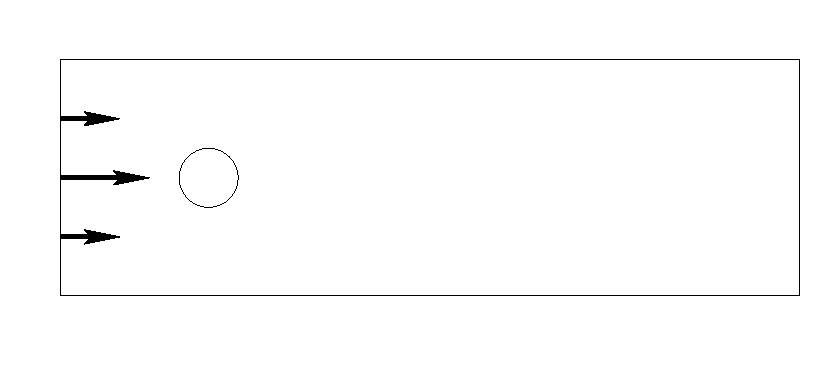
\includegraphics{Pictures/example_ns.pdf}%
\end{picture}%
\setlength{\unitlength}{4144sp}%
%
\begingroup\makeatletter\ifx\SetFigFontt\undefined%
\gdef\SetFigFontt#1#2#3#4#5{%
  \reset@font\fontsize{#1}{#2pt}%
  \fontfamily{#3}\fontseries{#4}\fontshape{#5}%
  \selectfont}%
\fi\endgroup%
\begin{picture}(6330,2785)(3136,-4652)
\put(9001,-4561){\makebox(0,0)[lb]{\smash{{\SetFigFontt{14}{16.8}{\familydefault}{\mddefault}{\updefault}{\color[rgb]{0,0,0}$(2.5,0)$}%
}}}}
\put(9001,-2086){\makebox(0,0)[lb]{\smash{{\SetFigFontt{14}{16.8}{\familydefault}{\mddefault}{\updefault}{\color[rgb]{0,0,0}$(2.5,0.41)$}%
}}}}
\put(3376,-2086){\makebox(0,0)[lb]{\smash{{\SetFigFontt{14}{16.8}{\familydefault}{\mddefault}{\updefault}{\color[rgb]{0,0,0}$(0,0.41)$}%
}}}}
\put(3376,-4561){\makebox(0,0)[lb]{\smash{{\SetFigFontt{14}{16.8}{\familydefault}{\mddefault}{\updefault}{\color[rgb]{0,0,0}$(0,0)$}%
}}}}
\put(7201,-3661){\makebox(0,0)[lb]{\smash{{\SetFigFontt{14}{16.8}{\familydefault}{\mddefault}{\updefault}{\color[rgb]{0,0,0}${\Omega}$}%
}}}}
\put(5851,-2086){\makebox(0,0)[lb]{\smash{{\SetFigFontt{14}{16.8}{\familydefault}{\mddefault}{\updefault}{\color[rgb]{0,0,0}$\Gamma_{wall}$}%
}}}}
\put(5851,-4561){\makebox(0,0)[lb]{\smash{{\SetFigFontt{14}{16.8}{\familydefault}{\mddefault}{\updefault}{\color[rgb]{0,0,0}$\Gamma_{wall}$}%
}}}}
\put(3151,-3211){\makebox(0,0)[lb]{\smash{{\SetFigFontt{14}{16.8}{\familydefault}{\mddefault}{\updefault}{\color[rgb]{0,0,0}$\Gamma_{in}$}%
}}}}
\put(9451,-3211){\makebox(0,0)[lb]{\smash{{\SetFigFontt{14}{16.8}{\familydefault}{\mddefault}{\updefault}{\color[rgb]{0,0,0}$\Gamma_{out}$}%
}}}}
\end{picture}%
}
\caption{Flow around a cylinder with 
circle-center $C=(0.2,0.2)$ and radius $r=0.05$.}
\label{fig:example_ns}
\end{figure}

We split the program into the parts \texttt{main.cc}, \texttt{func.h} and 
\texttt{pde.h}. The \texttt{main.cc}-file is responsible for the declaration 
of various objects which have mostly to do with the \textit{discretization}, 
the \textit{solvers} and the general \textit{program sequence}, whereas the 
other two contain most of the problem-data -- especially the cell-wise 
contributions of the weak form in \texttt{pde.h} and the functional in 
\texttt{func.h}. 
We give a brief explanation on every file in the following.

\subsubsection{\texttt{main.cc}}
In this file, we gather all the basic components that are necessary for the
solution process of a (stationary) partial differential equation. The
structure of the program is basically the same for every equation under
consideration, what changes is typically just the \textit{kind} of  finite
element or linear solver we want to use. Here, a key issue is that we only need to pick 
some pre-implemented routines from the \dope{} library rather than 
implementing these ourselves.


After the usual preamble, in which we include the necessary header-files 
from \deal{}, \dope{} and our own problem-data (i.e. \texttt{func.h} 
and \texttt{pde.h}), we start by defining an instance of a 
\texttt{ParameterReader}-object, which handles reading of run-time parameters.
\begin{lstlisting}
   ParameterReader pr;
\end{lstlisting}
The object \texttt{pr} then reads a text-file in which we might specify some 
problem-related parameters (for instance the viscosity $\nu$), but also general
 parameters for (non)-linear solvers and the output-format of computed data. 
After that, we create a triangulation of the domain $\Omega$ named 
\texttt{triangulation} using the tools provided by the \deal{} FE-library.

Next, we create some quadrature rules (for the evaluation of integrals over
cells \texttt{quad} and faces \texttt{face\_quad}) and a finite element \text{fe}
appropriate for the PDE at hand. We
choose a Gaussian quadrature of a certain degree and the previously mentioned
Taylor-Hood element. These routines are quite standard in each finite element
software and thus we can use those provided by the FE-library \deal{}.

Then, the two characteristic features \texttt{LocalPDE} and \texttt{LocalFunctional} objects come into play:
\begin{lstlisting}
  LocalPDE pde;
  LocalFunctional functional;
\end{lstlisting}
These hold the information of the PDE and the functional under consideration. Further explication is given below because
the definition of this classes is done separately in \texttt{pde.h} 
and \texttt{func.h} respectively.

In the next step, we define an object of type \texttt{SpaceTimeHandler}, which handles all the things connected with the triangulation as well as the finite element space. 
\begin{lstlisting}
  SpaceTimeHandler dof_handler(triangulation,
                               fe);
\end{lstlisting}

Now we have everything at hand to create an instantiation of the container for the problem data \texttt{PDEProblemContainer}. This basically represents the discretized problem, and bundles things like boundary conditions, the PDE, the functional and the discretization. First, we give the constructor the \texttt{pde} and the \texttt{dof\_handler}.
\begin{lstlisting}
  PDEProblemContainer<LocalPDE> 
             prob_container(pde, dof_handler);                                            
\end{lstlisting}
After that, we add the functional under consideration and, because it is a 
functional acting on the boundary, specify the part of the boundary on which 
the functional operates (this is done via a 'boundary color', where $1$ 
represents $\Gamma_{circ}$).
\begin{lstlisting}
  prob_container.AddFunctional(&functional);
  prob_container.SetBoundaryFunctionalColors(1);
\end{lstlisting}
Next, we incorporate the Dirichlet data. To this end, we instantiate a 
class \texttt{DirichletData} containing the required description of the 
boundary values. Then we have to tell the \texttt{prob\_container} for
which components and boundaries we prescribe the Dirichlet conditions. This is
done via a boundary-color and a so-called component mask 
(here, $0$ denotes $\Gamma_D$).
\begin{lstlisting}
  DirichletData dd;
  prob_container.SetDirichletBoundaryColors(0,
                                            comp_mask,
                                            dd);
\end{lstlisting}
Now, we create the object which steers the whole solution process, the previously mentioned \texttt{StatPDEProblem}. It takes care of solving the discretized equation and evaluating the given functionals. The class depends actually on some template-parameters, so for the sake of abbreviation, we defined a typedef at the beginning of the \texttt{main.cc}-file.
\begin{lstlisting}
  typedef StatPDEProblem<NEWTON> PDE;
\end{lstlisting}
Here, \texttt{NEWTON} itself is an abbreviation of
\begin{lstlisting}
  typedef NewtonSolver<LINSOLVE> NEWTON;
\end{lstlisting}
The  template parameter \texttt{LINSOLVE} describes which linear solver we use in this example. We opted for a direct solver, so: 
\begin{lstlisting}
  typedef DirectLinearSolver<MATRIX, VECTOR> LINSOLVE;
\end{lstlisting}
With the types settled, we create the object \texttt{solver}, which needs the discretization (represented here by the \texttt{prob\_container}), the parameter reader as well as the quadrature rules.
\begin{lstlisting}
  PDE pde(prob_container, pr,
                    quad, face_quad);
\end{lstlisting}
Finally, we compute the value $J(u_h)$ by calling:
\begin{lstlisting}
  pde.ComputeReducedFunctionals();
\end{lstlisting}
\todoww{Should we add a complete listing?}
\subsubsection{\texttt{pde.h}}
We shall now give an overview to the implementation of the specific form of the PDE. 

Let $N$ be the number of degrees of freedom of our discretization and $\Set{\phi_{h}^{i}|1\leq i \leq N}$ be a given FE-Basis. As stated in subsection~\ref{subsubsec:stationary problems}, to solve the discrete equation \eqref{eq:discrete_equation} we need the residual, i.e. the vector
\begin{align}\label{eq:discrete_residual}
\left(a(u_h)(\phi_{h}^{i})-(f,\phi_{h}^{i})\right)_{i=1}^N.
\end{align}
The corresponding Jacobian can be defined analogously.
Now, all we have to supply here are the cell-wise contributions to these terms,
then the \texttt{Integrator} object 
takes care of assembling \eqref{eq:discrete_residual}
and similarly of the matrix for the linearized equation to be solved.

To this end, we define a class \texttt{LocalPDE} which provides the three methods
\texttt{CellEquation}, \texttt{CellRightHandSide} and \texttt{CellMatrix}. 
The splitting of these terms is similar to Gascoigne
\cite{gascoigne} whereas the content (i.e., the 
implementation itself) of these
terms works as it is required by the FE-library for which the integration is done, here this is \deal{}.


We show the basic structure of these methods using the \texttt{CellEquation} 
method for the implementation of the cell-wise integrals.

\begin{lstlisting}
  void CellEquation(const CellDataContainer &cdc,
                    VECTOR &local_vector)
  {
    const auto& fe_values = cdc.GetFEValuesState();
    unsigned int dofs_per_cell = cdc.GetNDoFsPerCell();
    unsigned int n_q_points = cdc.GetNQPoints();
\end{lstlisting}
 The \texttt{CellDataContainer} contains all the information we need to compute the cell-contributions (things like number of quadrature points, number of degrees of freedom on the cell, the \texttt{dealii::FEValues}-objects, etc.).
To get access to the values and the gradient of the solution in the quadrature 
points we need to extract them from the \texttt{CellDataContainer}:
\todoww{Ich habe jetzt das Arg. in state ge\"andert, das wollten wir sowieso in 
\dope{} umsetzen und ist dann nicht so umst\"andlich}
  \begin{lstlisting}
    cdc.GetValuesState("state", uvalues);
    cdc.GetGradsState("state", ugrads);
 \end{lstlisting}
 In these two lines, we load the values and the gradient of the solution 
during the last Newton iteration in all the quadrature points on the cell 
into the two variables \texttt{uvalues} and \texttt{ugrads}.

In the next lines, we finally implement our concrete 
cell contribution of the PDE. Thus,
we loop over the quadrature points and the number of DoFs of the cell. In the innermost loop, we evaluate the weak form tested with $\phi_{h}^i$ (here \texttt{phi\_i\_grads\_v} denotes the matrix $\nabla \phi_h^i$) 
on the cell with the help of the previously selected quadrature formula. 
 \begin{lstlisting}
    for(unsigned int q_point = 0; 
        q_point < n_q_points; 
        q_point++)
    {
      //initialize phi_i_grads_v etc.
      Tensor<2,2> vgrads;
      vgrads[0]= ugrads[q_point][0]; 
      vgrads[1]= ugrads[q_point][1];
      for (unsigned int i=0;i<dofs_per_cell;i++)
        local_vector(i) += 
           ( _nu * vgrads * phi_i_grads_v 
             + //all the other terms
           ) * fe_values.JxW(q_point);
    }
\end{lstlisting}
\dope{} takes care of the distribution of the local cell contributions into  the vector of the residual \eqref{eq:residual_vector}. The methods \texttt{CellRightHandSide} and \texttt{CellMatrix} follow the same structure as 
\texttt{CellEquation}, so we do not go into the details here.

\subsubsection{\texttt{func.h}}
The implementation of the boundary-functional $J$ follows the outline of the
computation of the cell-residual in \texttt{pde.h}. 
The main difference, and common to all functionals, is that as we only want 
to evaluate a functional, i.e. a number, and not a residual-vector. 
Hence, we loop over the quadrature points and not over the local 
degrees of freedom. 

In the present situation, we want to evaluate a functional 
that consists of a boundary integral. Thus we need to evaluate 
integrals on faces, those who lie on $\Gamma_{circ}$, instead of integrals over
cells. 
This face contributions are calculated in \texttt{BoundaryValue} and added to 
sum up to the value of $J$. 
\begin{lstlisting}
 double
 BoundaryValue(const FaceDataContainer& fdc)
  {
    //same as before, get n_q_points etc.
    const auto& face_values = fdc.GetFEFaceValuesState();
    fdc.GetFaceValuesState("state", ufacevalues);
    fdc.GetFaceGradsState("state", ufacegrads);
    
    double erg = 0.;
    for(unsigned int q_point = 0; 
        q_point < n_q_points; 
        q_point++)
      erg -= ( _nu * ufacegrads[q_point][0]
               * face_values.normal_vector(q_point)
               + //other terms        
             ) * face_values.JxW(q_point);
    return erg;
  }
\end{lstlisting}

\subsection{Solving Nonstationary PDEs}\label{sec:timedep}
To describe the solution of nonstationary 
PDEs, we consider a time-dependent semi-linear form $a(u)(\phi)$ and some
right hand side functional $l$. Let $I:=[0,T]$ be a time interval with end time point value $T$.
The weak for of such a problem then consists of finding some $u$ such that
\[
\int_I \overline{a}(u)(\phi)\, dt = \int_I l(\phi)\, dt \quad \forall\Phi\in X,
\]
with some suitable Bochner space $X$.  As model problem,
we extend the previous example and consider the nonstationary Navier-Stokes equations
in a spatial domain $\Omega\in\mathbb{R}^d$. The weak for is then to find 
$u = (v,p)\in X$ with
\begin{align*}
&\int_I \bigl[ (\partial_t v, \phi)
+ \nu (\nabla v, \nabla \phi) + (v\cdot\nabla v, \phi)
- (p,\nabla\cdot \phi)
+ (\nabla\cdot v, \chi)\bigr] \, dt\\
&\quad + (v(0) - v^0, \phi(0))
= \int_I (f,\phi) \, dt 
\end{align*}
for all $\Phi:= (\phi, \chi) \in X$ with
\[
X:= \set{ 
(v,p) | v\in L^2(I,H_0^1(\Omega)^d) , 
\partial_t v\in L^2(I, L^2(\Omega)^d), 
p\in L^2(I,L^2(\Omega)\setminus\mathbb{R})}.
\]
We note that the only difference is the appearance of an additional
time integration, the initial-value, and the term 
\[
\int_I (\partial_t v, \phi)\,dt
\]
so that we can reuse our stationary implementation for all the other 
terms if we rescale them appropriately in the time integration.

As for stationary problems, the goal is to compute
some target functional $J$ which is now possibly 
time-dependent. To organize the discretization 
process, we need to perform spatial and temporal 
discretization. This is again done via
an object that takes care of organizing the degrees of 
freedom, as in the case of stationary problems.
The only difference to the stationary case is that we need to 
add the temporal subdivision \texttt{times}. In the simplest 
case, when we have the same spatial triangulation 
at all times, the constructor could look as follows:
\begin{lstlisting}
  template<typename TIMES, typename TRIANGULATION, 
           typename FE>
   void SpaceTimeHandler(TIMES& times,
                         TRIANGULATION& triag,
                         FE& fe);
\end{lstlisting}

Now we may discretize the problem with some time-stepping scheme, which will 
remove the temporal derivative and replace it by some difference quotients. 
Since the exact way of doing this depends on the time-stepping scheme 
we need a new object that takes the user-given description of the PDE and 
generates the appropriate combinations of spatial integrals and scaling.
Thus a generic problem may look as follows:
\begin{lstlisting}
  template<typename PROBLEM>
      class TimeStepProblem(Problem & P);
\end{lstlisting}
At present we have prepared the following time-stepping schemes in \dope:
\begin{itemize}
\item Forward-(or Explicit)-Euler
\item Backward-(or Implicit)-Euler
\item Crank-Nicolson scheme
\item Shifted Crank-Nicolson scheme (to deal with singular initial data)
\item Fractional-Step-$\theta$ scheme
\end{itemize}
After choosing the time-stepping scheme, the \texttt{SpaceTimeHandler}  
loops over all time-steps, where in each of the 
time-steps we can reuse the functionality we have provided to solve 
stationary PDEs. 
This means for instance, if we have implemented the 
cell-integrals in the weak formulation for the stationary case, 
then we can use the exact same 
implementation again for the solution of the nonstationary version of 
the equation. However, we need to provide an additional 
term to cope with the integral for the time derivative.

Now it is apparent, why we introduced the \texttt{StatPDEProblem}, because
we define the \texttt{InstatPDEProblem} to contain the necessary 
loop over all time points. Consequently, the implementation 
of nonstationary problems is quite similar to stationary problems,
at least from the user implementation point of view,
which was one major goal we claimed at the beginning.
Next, we will describe the methods the user needs to 
provide in addition to the stationary case.

\subsubsection{Problem-Dependent 
Implementation of Nonstationary Problems}
\label{sec:timedep:implementation}
We explain in more detail the temporal discretization
and specific issues of its implementation. 
To keep the presentation easy, we neglect
all material coefficients
to give the idea based on the weak 
form of the Navier-Stokes equations:
Find $(v,p)$ such that for all $(\phi,\chi)$ 
and all $t \in I$
\begin{align*}
(\partial_t v,\phi) 
+ (\nabla v, \nabla \phi)
+ (v\cdot\nabla v,\phi)
-(p,\nabla\cdot \phi)
+(\nabla\cdot v, \chi)
=(f,\phi),
\end{align*}
where $f$ describes some volume forces.
Temporal discretization using the One-step-$\theta$ scheme reads:
Given the old time-step solution $(v^n,p^n)$, 
find $(v^{n+1}, p^{n+1})$ (and multiplication 
by the inverse of the time-step $k$):
\begin{align*}
(v^{n+1} - v^{n}, \phi)
&+ k\theta (\nabla v^{n+1}, \nabla \phi)
+ k\theta (v^{n+1}\cdot\nabla v^n + 
  v^{n}\cdot\nabla v^{n+1},\phi)\\
&- k (p^{n+1},\nabla\cdot \phi)
+ k(\nabla\cdot v^{n+1}, \chi)\\
=&\; k\theta (f^{n+1},\phi) + k(1-\theta) (f^{n},\phi)
- k(1-\theta) (\nabla v^{n}, \nabla \phi) 
\end{align*}
The concrete choice of $\theta$ leads to a
specific time-stepping scheme. For instance,
$\theta = 0.5$ gives the Crank-Nicolson scheme.

It is well-known in fluid mechanics that the pressure and incompressibility terms should be 
treated fully implicitly when time-discretizing 
the Navier-Stokes equations.
For this reason, the implementation is split up
into several items to account for fully implicit 
terms and remaining terms for which we need 
old time-step and present time-step values. 
Hence, in the local cell equation, the parameters
\texttt{scale} and \texttt{scale\_ico}
are used to distinguish these terms.
I the present context this means that 
\texttt{scale} $= \pm k\theta$ or \texttt{scale} $= \pm k(1-\theta)$ and
\texttt{scale\_ico}~$= \pm k$.

With this the \texttt{CellEquation} needs to contain the terms weighted
with the appropriate scaling as it is indicated below but is otherwise the 
same as it is in the stationary case. 
\begin{lstlisting}
  void CellEquation(...)
   {
   // Usual loops over DoFs and quadrature points
     {
      local_cell_vector(i) += 
         scale * 
         // terms like (\nabla v^{n+1}, \nabla\phi) etc.
        + scale_ico *
         // terms like (-p^{n+1},\nabla\cdot\phi)
     }
   }
\end{lstlisting}
Analogous procedure is performed in the local 
cell matrix.
\begin{remark}
Note that in the stationary case there is no such difference and accordingly 
\dope{} automatically sets $ \texttt{scale\_ico} = \texttt{scale}$, so that in fact the user has to implement the \texttt{CellEquation} only once and can henceforth reuse it in all his stationary and nonstationary problems if 
\texttt{scale} and \texttt{scale\_ico} are properly used. 
This transfers of course also to other methods like \texttt{CellMatrix}.
\end{remark}

In comparison to stationary problems, we need to consider, in addition, 
the implementation
of the time-derivative, i.e., the term $ (v^{n+1},\phi)$. This is done
in the method \texttt{CellTimeEquation} in a straight-forward way. After the initialization of $\texttt{v}$ and the shape function $\texttt{phi\_i}$ and the usual loops over the quadrature points and  degrees of freedom of the cell we fill the local cell vector by
\begin{lstlisting}
    local_cell_vector(i) +=  scale * (v * phi_i)  
                             * fe_values.JxW(q_point);    
\end{lstlisting}
Here, the advantage is that \dope{} orders the terms in the time-stepping
problems
such that only $(v^{n+1},\phi)$ must be implemented. 



\begin{remark}[Nonlinear terms in the time derivative]
However, if someone 
needs to give an explicit formula for the difference quotient
this can be written using the methods
\begin{lstlisting}
  void CellTimeEquationExplicit (...)
   {
     // implement (v^{n+1},\phi) and (v^n,\phi)  
   }
\end{lstlisting}
Such explicit statements may be useful for nonlinear terms to which time 
derivatives are applied as it appears for instance in fluid-structure 
interaction problems.
\end{remark}

\begin{remark}[Fractional-Step-$\theta$-scheme]
The temporal discretization in this section 
is based on the One-Step-$\theta$-schemes. The library
offers in addition an implementation 
of the second-order and strongly $A$-stable 
Fractional-Step-$\theta$-scheme in which 
each time-step is subdivided into three 
sub-steps. However, no additional implementation is needed by the user 
for the application of the Fractional-Step-$\theta$-scheme.
\end{remark}

\subsection{Solving Optimization Problems}\label{sec:opt}
Once we are able to solve stationary and nonstationary PDEs
we can consider optimization problems constrained by these PDEs.
How this is done will be described in this section. 

A prototypical PDE constrained optimization problem reads:
\begin{align*}
\min\;&J(q,u) \\
  &\text{s.t.}\; a(q,u)(\phi) = 0 \quad \forall \phi\in V,\\
  &q_- \le q \le q_+,\\
  &g(q,u) \le 0,  
\end{align*}
where $u$ is a function and $q$ can either be a function or some 
fixed number of parameters. the numbers $q_-$ and $q_+$ are bounds for 
the control $q$, and $g(\cdot)$ is some state constraint.
To keep the presentation brief we will neglect the additional bounds
\[
a \le q \le b,\qquad g(q,u) \le 0
\]
although they can be treated by \dope{} as well.
Then, in order to minimize the functional $J$ one may apply the, so-called, 
reduced approach, in which we eliminate the dependent variable $u$ by the solution 
operator $S$ of the (stationary or nonstationary) PDE, i.e., 
\begin{align*}
a(q,S(q))(\phi) = 0 \quad \forall \phi\in V. 
\end{align*}
Thus replacing $u$ by $S(q)$ one is left with the problem
\begin{align*}
\min\;&j(q) = J(q,S(q)). 
\end{align*}
This can be discretized using the finite element approximation $S_h$ of $S$ 
and yields the problem 
\begin{align*}
\min\;&j_h(q) = J(q,S_h(q)). 
\end{align*}
After possibly discretizing the control $q$ as well using finite elements, 
one can apply any algorithm to solve the, unconstraint, minimization 
problem. This, will in any case require the evaluation of $j_h(q)$ which 
we can do, e.g., using \texttt{StatPDEProblem::ComputeReducedFunctional} for 
a stationary PDE or using \texttt{InstatPDEProblem::ComputeReducedFunctional} 
for nonstationary PDEs. 

If one would like to use derivative based methods, one 
needs, in addition, derivatives of $j_h$ and thus of $J$ as well as of $S_h$. 
We remark, that one can calculate the derivative of 
$j$ using adjoint calculus. Then the directional derivative 
of $j$ in direction $\delta q$ is given by
\[
j'_h(q)(\delta q) = J'_q(q,S_h(q))(\delta q) + (S_h^* J_u'(q,S_h(q)),\delta q)
\]
where the index $q$ or $u$ denote directional derivatives for the 
respective argument. To calculate the action of the adjoint operator $S_h^*$ 
we note that $z =  S_h^* J_u'(q,S_h(q))$
can be computed via the adjoint PDE
\begin{equation}
  \label{opt_KKT_system}
  \begin{aligned}
    a_{u}'(q,u)(\phi , z) &= J'_{u}(q,u)(\phi) & \forall \phi&\in {\cal X}.
  \end{aligned}
\end{equation}
Similarly formulas for the second derivatives can be obtained, see, e.g., 
\cite{BeMeVe06}.

We define an object 
\begin{lstlisting} 
  template<typename PDE, typename COSTFUNCTIONAL>
    class OPTProblemContainer;
\end{lstlisting}
that collects the user given PDE and functional descriptions and constructs the 
required PDE and right hand side information needed for the calculations.

This means, for solving optimization problems with PDEs, the user needs to
provide the derivatives of the functional and the PDE 
in addition to the already defined functions \texttt{CellEquation}, 
\texttt{BoundaryValue}. For the above adjoint equation these are 
\begin{lstlisting} 
  void CellEquation_U(...)
   {
     // implement directional derivative 
     // of the CellEquation w.r.t. u
   }
\end{lstlisting}
and functional terms, i.e.,     
\begin{lstlisting} 
  void BoundaryValue_U(...)
   {
     // implement here the derivative of 
     // the boundary cost functional w.r.t. u
   }
\end{lstlisting}

Based on this classes we can now solve the optimization problem, for instance using 
a Newton type method for the reduced problem, see, e.g., \cite{NoWr00}. This yields 
an object \texttt{ReducedNewtonAlgorithm} which needs to be initialized 
with the \texttt{OptProblemContainer} and then provides 
the following method to be called by the user
\begin{lstlisting}
  ReducedNewtonAlgorithm::Solve(ControlVector<VECTOR>& )
\end{lstlisting}
where the argument provides an initial guess for the optimal control.

Summarizing, we learned from the previous sections 
that 
due to the design of the classes it is easily possible to extend any given 
and running code for a PDE both to the nonstationary counterpart, if the PDE is 
stationary, as well as to an optimization problem where the constraint is 
given by this PDE. Meaning that the use of our framework for the simulation of 
PDEs will, due to the enforced interface, enable easy application of state-of-the-art 
optimization algorithms to minimization problems governed by the PDE.


\subsection{Additional Features}\label{sec:additional}
Finally, we shall give a brief summary of features 
that are applicable (in general) to all types of problems. Specifically,
\dope{} provides goal-oriented mesh refinement with the help of the 
Dual Weighted Residual (DWR) method, see \cite{BeRa96} or \cite{BR03}. Here, a 
given cost functional such as a point evaluation, line integration or domain
integration is considered as target quantity. 
The same routines 
can also be used, without any modification by the user, to use standard 
residual error estimators by exchanging the 
error estimator class.

Since in many applications it is desirable to use different discretizations
for the state and the control \dope{} provides multi-mesh support, meaning that
once a problem has been written correctly using the same mesh for all finite element
variables one can switch to a different SpaceTimeHandler that allows different meshes for all 
variables without the need to change the user-given implementation of the PDE and functional.

%%%%%%%%%%%%%%%%%%%%%%%%%%%%%%%%%%%%%%%%%%%
\section{Applications}
\label{applications}
In this final section, 
we present three numerical tests which demonstrate different
features of \dope{}:
\begin{itemize}
\item In the first numerical example, we consider 
goal-oriented mesh refinement with the help of the 
DWR method for the stationary Navier-Stokes equations.
\item The second example presents nonstationary fluid-structure 
interaction. The challenges for those kind of problems are the multi-domain
character of the coupled problem and the treatment of the coupling conditions.
The problem is formulated in a variational monolithically-coupled way which 
allows to consider goal-oriented mesh refinement and gradient-based optimization.
\item In the third numerical test, an optimization problem for structural mechanics
is discussed.
\end{itemize}

\subsection{Goal-Oriented Mesh Refinement for Navier-Stokes}
In this example, we consider a laminar flow around a cylinder in 2d. To be more precise, we are computing the benchmark 2D-1 from \cite{TuSchae96}. The computational domain is as depicted in Fig.~\ref{fig:example_ns} and the equation is discretized with the Taylor-Hood  element. We want to compute the drag force on the enclosed cylinder
\begin{equation}
J(u) = \frac 1 {20} \int_{\Gamma_{circ}} \nu\partial_nv _1 - pn_1,
\end{equation}
with the solution $u = (v,p)$, the normal $n$ and the viscosity $\nu = 0.001$.
\begin{figure}[hbt]
\centering
{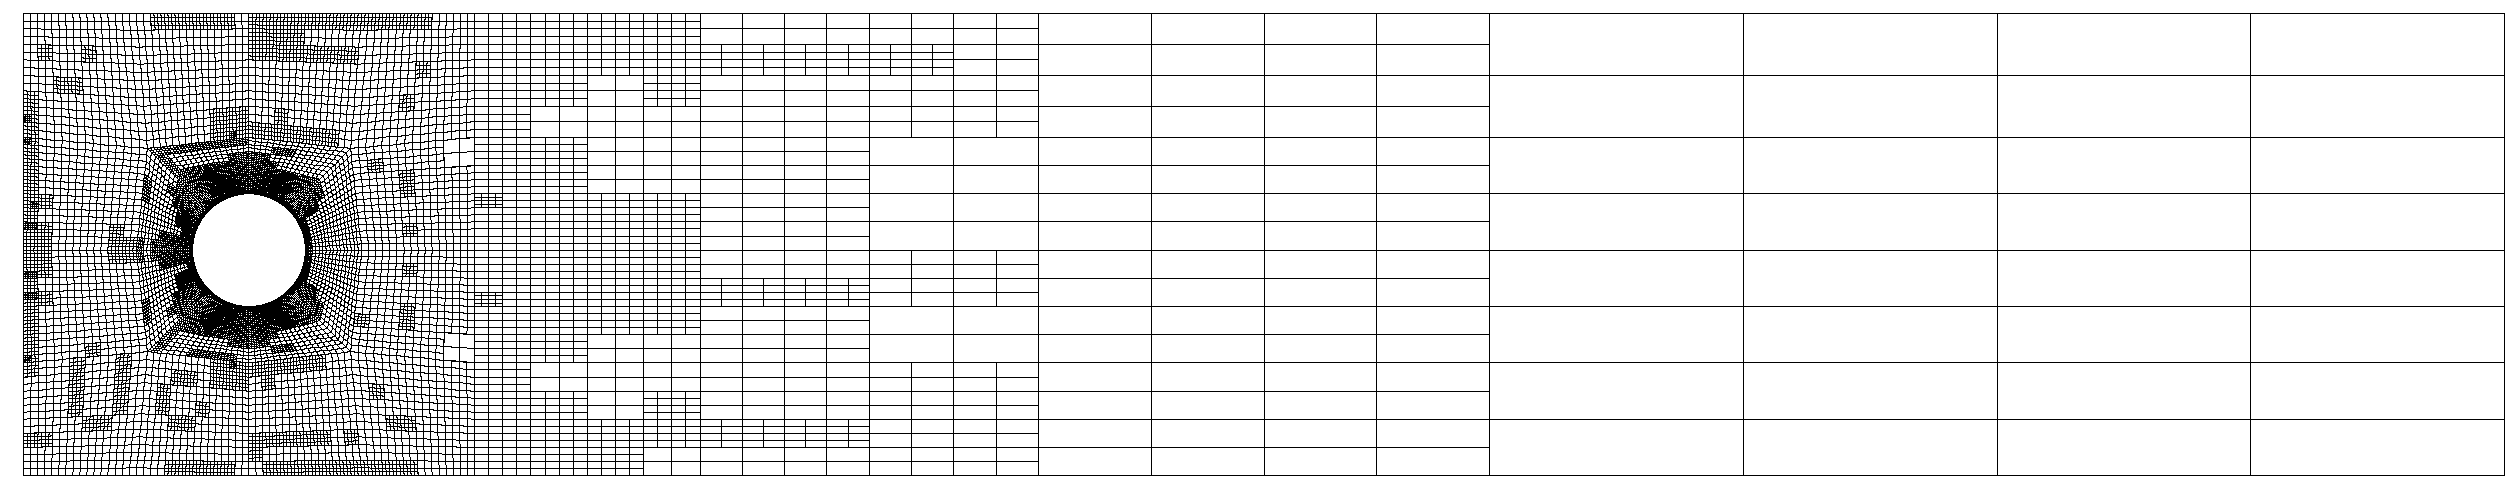
\includegraphics[width=0.9\textwidth]{Pictures/local_grid_NS.png}}
\caption{Locally adapted grid after eight refinement steps.}
\label{fig:NS_local_grid}
\end{figure}
To achieve an efficient computation of the quantity $J$, we employ goal-oriented mesh refinement with the help of the DWR-method, see \cite{BeRa96}. The method delivers error indicators and by this way computational grids tailored to minimize the error in the previously given functional $J$. The price we have to pay is the additional computation of a (linear) dual problem, which is implemented as described in Section~\ref{sec:opt}. In Fig.~\ref{fig:NS_local_grid} we see a resulting triangulation after eight refinement steps with roughly $320\,000$ degrees of freedom.

In Fig.~\ref{fig:NS_comparison} we compare the errors in the functional obtained by using global and local mesh refinement. We see clearly that the local mesh refinement allows for substantial savings with respect to degrees of freedom.

\begin{figure}[hbt]
\centering
\resizebox{0.5\textwidth}{!}{\begin{picture}(0,0)%
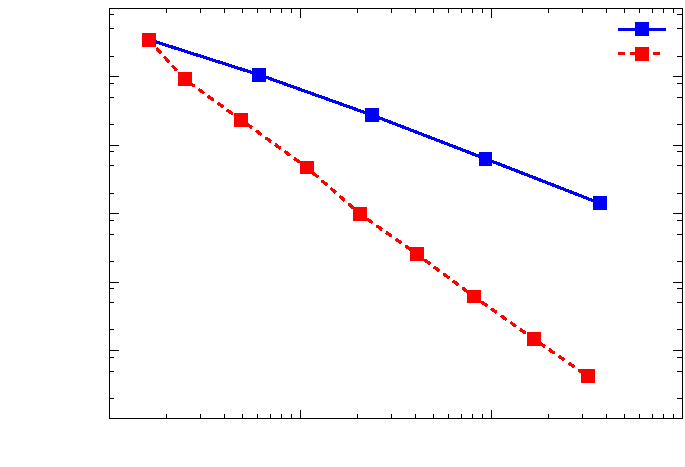
\includegraphics{Pictures/ConvergenceNS.pdf}%
\end{picture}%
\setlength{\unitlength}{4144sp}%
%
\begingroup\makeatletter\ifx\SetFigFont\undefined%
\gdef\SetFigFont#1#2{%
  \fontsize{#1}{#2pt}%
  \selectfont}%
\fi\endgroup%
\begin{picture}(5212,3544)(911,-3686)
%  Begin plot #1 
 \put(5560,-403){\makebox(0,0)[rb]{\smash{{\SetFigFont{12}{14.4}global}}}}
% %  Begin plot #2 
 \put(5560,-590){\makebox(0,0)[rb]{\smash{{\SetFigFont{12}{14.4}local}}}}
 \put(1680,-3372){\makebox(0,0)[rb]{\smash{{\SetFigFont{12}{14.4}$10^{-6}$}}}}
 \put(1680,-2850){\makebox(0,0)[rb]{\smash{{\SetFigFont{12}{14.4}$10^{-5}$}}}}
 \put(1680,-2329){\makebox(0,0)[rb]{\smash{{\SetFigFont{12}{14.4}$10^{-4}$}}}}
 \put(1680,-1807){\makebox(0,0)[rb]{\smash{{\SetFigFont{12}{14.4}$10^{-3}$}}}}
 \put(1680,-1286){\makebox(0,0)[rb]{\smash{{\SetFigFont{12}{14.4}$10^{-2}$}}}}
 \put(1680,-764){\makebox(0,0)[rb]{\smash{{\SetFigFont{12}{14.4}$10^{-1}$}}}}
 \put(1680,-243){\makebox(0,0)[rb]{\smash{{\SetFigFont{12}{14.4}$10^{0}$}}}}
 \put(1744,-3579){\makebox(0,0)[b]{\smash{{\SetFigFont{12}{14.4}$10^{3}$}}}}
 \put(3199,-3579){\makebox(0,0)[b]{\smash{{\SetFigFont{12}{14.4}$10^{4}$}}}}
 \put(4653,-3579){\makebox(0,0)[b]{\smash{{\SetFigFont{12}{14.4}$10^{5}$}}}}
 \put(6108,-3579){\makebox(0,0)[b]{\smash{{\SetFigFont{12}{14.4}$10^{6}$}}}}
 \put(1012,-1755){\rotatebox{-270.0}{\makebox(0,0)[b]{\smash{{\SetFigFont{12}{14.4}${J}(u-u_h)$}}}}}
 \put(3926,-3789){\makebox(0,0)[b]{\smash{{\SetFigFont{12}{14.4}\# Degrees of Freedom}}}}
\end{picture}%
}
\caption{Comparison of global and local mesh refinement with respect to the error in the drag-functional $J$.}
\label{fig:NS_comparison}
\end{figure}




\subsection{Nonstationary Fluid-Structure Interaction}
In this example, a challenging benchmark FSI 2
proposed by Hron and Turek \cite{HrTu06b} is considered.
To solve this problem accurately, it is very important that 
the coupling conditions
\[
v_f = v_s \quad \text{and} \quad \sigma_f n_f = \sigma_s n_s, 
\]
namely, the continuity of velocities and continuity of normal stresses
are satisfied in each time-step. This is achieved with the help of 
a monolithic coupling scheme (strong coupling).

The basic configuration is 
sketched in Fig.~\ref{fig:example_ns} at which an elastic beam is attached 
behind the rigid cylinder. 
The elastic beam has length
$l=0.35m$ and height $h=0.02m$. The right lower end is positioned at 
$(0.6m,0.19m)$, and
the left end is attached to the circle. 
Control points $A(t)$ (with $A(0) = (0.6,0.2)$) are fixed at the 
trailing edge of the structure, measuring $x$- and $y$-deflections of the beam.

Details 
on parameters and evaluation functionals and other results 
can be found in \cite{HrTu06b,BuSc06,DeHaeAnnBrVie10,Wi11}. 
The Fractional-Step-$\theta$ scheme is used for time discretization with
different time step sizes $k$. However, the time-stepping scheme can be 
very easily chosen in the \texttt{main.cc} function by choosing an appropriate 
time-stepping scheme as previously explained.

The quantities of interest are evaluations of 
$x$- and $y$ displacement at the point $A(0) = (0.6,0.2)$
and the drag and lift forces acting on the cylinder and the elastic beam:
\begin{align}
\label{drag_lift_forces}
(F_D , F_L) 
= {\int_{S_f} \sigma_f \cdot n_f \, ds + 
\int_{\Gamma_i} \sigma_s \cdot n_s \, ds},
\end{align}
where $S_{f}$ denotes the path over the cylinder in the fluid part and
$\Gamma_i$ the interface between the elastic beam and the 
fluid.

Since the problem is fully nonstationary, the 
dynamics are presents in Fig.~\ref{res:fsi_2_mesh_and_x_velo}. 
By comparison of our findings in Fig.~\ref{res:results_ux_and_uy_fsi_2}
with the literature, it can be identified that 
the implementation in \dope{} is correct.



% Bilder von FSI 2 
\begin{figure}[h]
\centering
{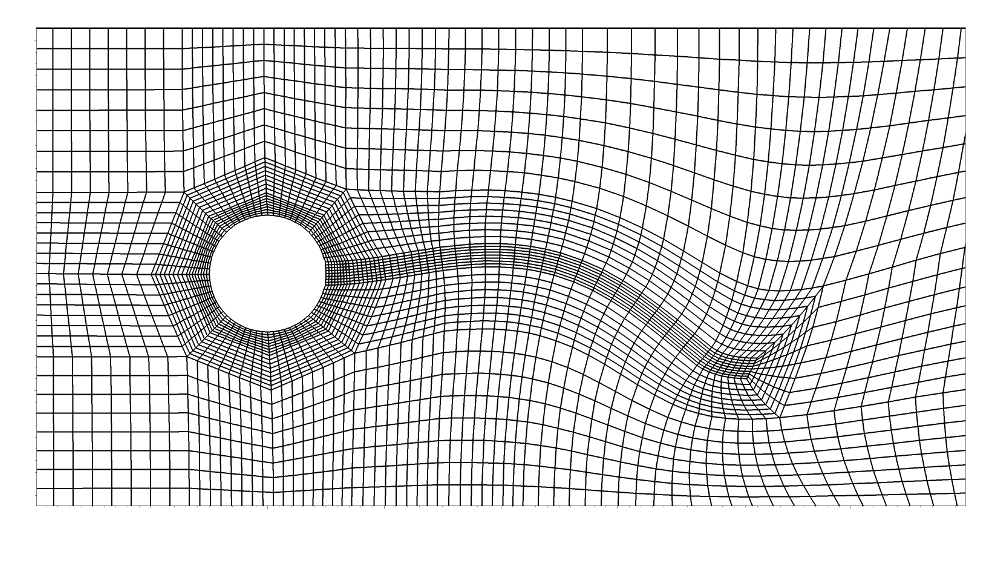
\includegraphics[width=5cm]{Pictures/visit_fsi_2_CNn_t_2e-2_global_3_biharmonic_mesh8070_scale.png}}
{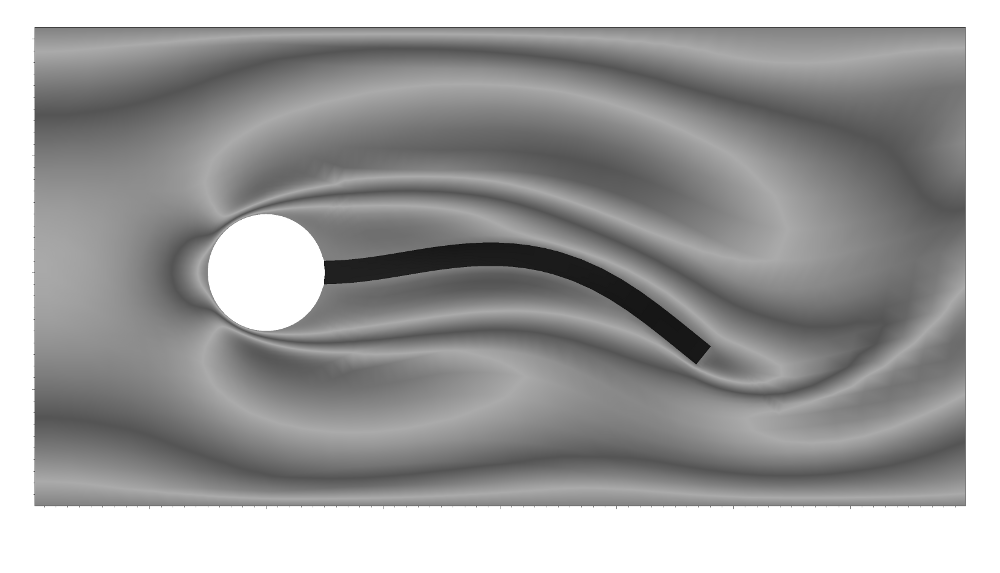
\includegraphics[width=5cm]{Pictures/visit_fsi_2_CNn_t_2e-2_global_3_biharmonic_x_velo8070_scale.png}}
\caption{FSI 2 test case: mesh (left) and velocity profile in vertical 
direction (right) at time $t=16.14s$.}
\label{res:fsi_2_mesh_and_x_velo}
\end{figure}

\begin{figure}
\centering
{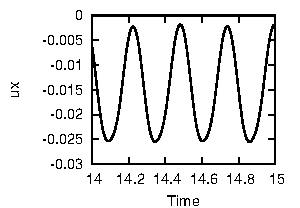
\includegraphics[width=5.8cm]{Pictures/ux_FSI_2_FS_t_3e-2_t_15e-3_global_2_Hron_grid.pdf}}
{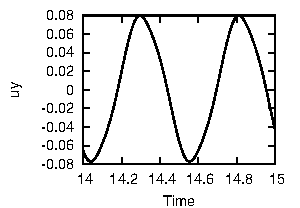
\includegraphics[width=5.8cm]{Pictures/uy_FSI_2_FS_t_3e-2_t_15e-3_global_2_Hron_grid.pdf}}
{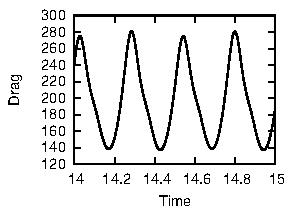
\includegraphics[width=5.8cm]{Pictures/Drag_fluid_FSI_2_FS_t_3e-2_t_15e-3_global_2_Hron_grid.pdf}}
{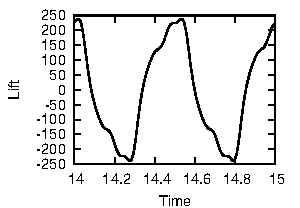
\includegraphics[width=5.8cm]{Pictures/Lift_fluid_FSI_2_FS_t_3e-2_t_15e-3_global_2_Hron_grid.pdf}}
\caption{FSI 2: the deflections of the beam, $u_x(A)$ and $u_y(A)$ (in $cm$), and 
the drag $F_D$ and the lift $F_L$ evaluation (in $kg/m\,s^2$) are displayed versus
time (in $s$).
} 
\label{res:results_ux_and_uy_fsi_2}
\end{figure}


\newpage
\subsection{Compliance Minimization}
In this example, we consider the compliance minimization of a standard MBB-Beam (Messerschmidt-B\"olkow-Blohm-Beam), see, e.g.,~\cite{BendsoeSigmund:2003}.
The thickness variable is allowed to take intermediate value apart from $0$ and $1$,
i.e., we consider a variable thickness sheet. The discretization is done 
using $Q_2$ elements for the displacement and discontinuous $P_0$ elements for the 
thickness.
\begin{figure}
\centering
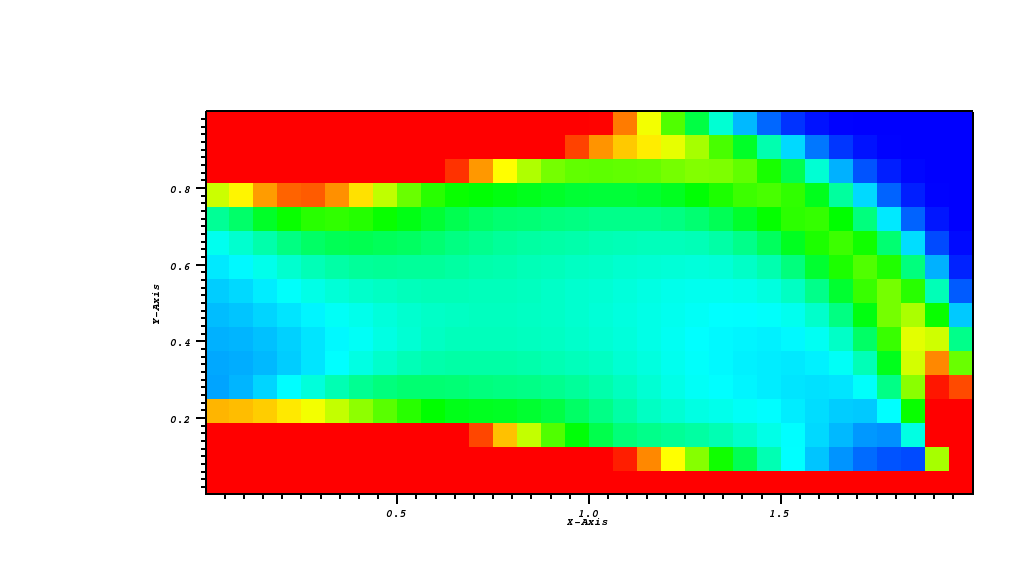
\includegraphics[width=1.\textwidth, viewport=205 88 975 500, clip]{Pictures/MBB.png}
\caption{Thickness distribution for the MBB-beam minimum compliance problem.} 
\label{res:mbb}
\end{figure}
A typical thickness distribution is shown in Fig.~\ref{res:mbb}.

\section{Conclusions}
In this article, we described the architecture 
of the novel software library \dope{} for solving 
PDEs and optimization problems.  The key idea of the software is to supply a
toolkit which allows for fast implementation of the problems at hand, but at
the same time gives the user full flexibility to change or alter the used
algorithms. 
This is achieved by a unified interface 
to state of the art time-stepping methods, nonlinear solvers and optimization
routines. The capabilities of \dope{} are demonstrated with the help of three examples.


\section*{Thanks}
The \dope{} project makes use of various finite elements taken from  
the \deal{} \cite{dealnew} finite element library which has been developed
 initially by W. Bangerth, R. Hartmann, and G. Kanschat \cite{dealold}.
The authors acknowledge their past experience as well as discussions 
on modularization of algorithms
with 
the authors of the libraries 
Gascoigne/RoDoBo project, which was initiated by 
Roland Becker, Dominik Meidner, and Boris Vexler \cite{rodobo}. 
Finally, the second author thanks Mary F. Wheeler (ICES, Austin) for the 
possibility to finish this work.

%%%%%%%%%%%%%%%%%%%%%%%%%%%%%%%%%%%%%%%%%%%
%\bibliographystyle{abbrvnat}
\bibliographystyle{acmsmall}
\bibliography{lit}
%



\end{document}
% end of file template.tex



